\section*{S12. Crossed population-model and pair-selection sensitivity}
The common domain contains 1,754,190 native GHSL pixels and 22,357,666.843 GHSL population units; 142,949.221 GHSL units from the full primary footprint are excluded. It intersects the primary footprint with full coverage of GHSL 2020 and WorldPop 2020 only; the four-layer epoch comparison in S6 uses a separately defined intersection. Each model is normalized to the GHSL total in this two-model domain before any support calculation. We cross these two allocations with the original 28-pair and expanded 224-pair mean joint support fields, at $q=0.3$. Neither population product is treated as demographic truth.

All comparisons use 1-km cells in UTM zone 47N and offsets $(0,0)$, $(500,0)$, $(0,500)$ and $(500,500)$ m. Within each combination, native-model and uniform allocations have identical cell population totals and the same included-domain area. We project extensive area, supported area, population and supported population separately onto a 50-m integration grid. The population--support product is formed before projection. Retaining partial cells avoids full-cell extrapolation outside the domain.

\begin{table}[htbp]\centering\footnotesize
\caption{Crossed population-model and pair-selection comparison at 1 km and $q=0.3$. Both models use the same domain and total. Deficits and differences are in millions of allocation units (M). Ranges span four grid origins; they are not confidence intervals. $\Delta=U_{\rm uniform}-U_{\rm native}$, and pp denotes percentage points of the common total.}\label{tab:cross}
\setlength{\tabcolsep}{3.5pt}
\begin{tabular}{llrrrrr}\toprule
Model & Pairs & Native (M) & Uniform (M) & $\Delta$ (M) & $\Delta$/native (\%) & $\Delta$/total (pp)\\\midrule
GHSL & 28 & 2.989 & 4.645--4.653 & 1.656--1.663 & 55.38--55.64 & 7.40--7.44\\
GHSL & 224 & 3.268 & 4.944--4.951 & 1.676--1.683 & 51.29--51.51 & 7.50--7.53\\
WorldPop & 28 & 5.186 & 5.654--5.657 & 0.468--0.471 & 9.03--9.07 & 2.09--2.10\\
WorldPop & 224 & 5.488 & 5.963--5.965 & 0.474--0.476 & 8.64--8.68 & 2.12--2.13\\
\bottomrule\end{tabular}\end{table}

Production first and cross moments conserve source totals to relative tolerance $10^{-8}$, and aggregation over each origin preserves those projected totals. Direct native-grid integration agrees with the coarse cross-moment reference. The 25-m diagnostic retains raw reprojection drift without renormalization (maximum absolute relative moment drift 1.65e-05). Its maximum change in uniform-minus-native difference is 0.000436 percentage points of the common total, below the prespecified 0.01-percentage-point numerical tolerance. These are numerical sensitivity checks, not uncertainty intervals.

All 16 production rows have positive uniform-minus-native differences. GHSL gives a larger effect than WorldPop under both pair selections. The result supports a persistent direction for these selected inputs, while showing that a single percentage cannot represent population-model sensitivity. Because pair number and pair composition change together, no causal effect of sample size is inferred. The four origins are deterministic sensitivity cases, not independent replicates.

\begin{figure}[htbp]\centering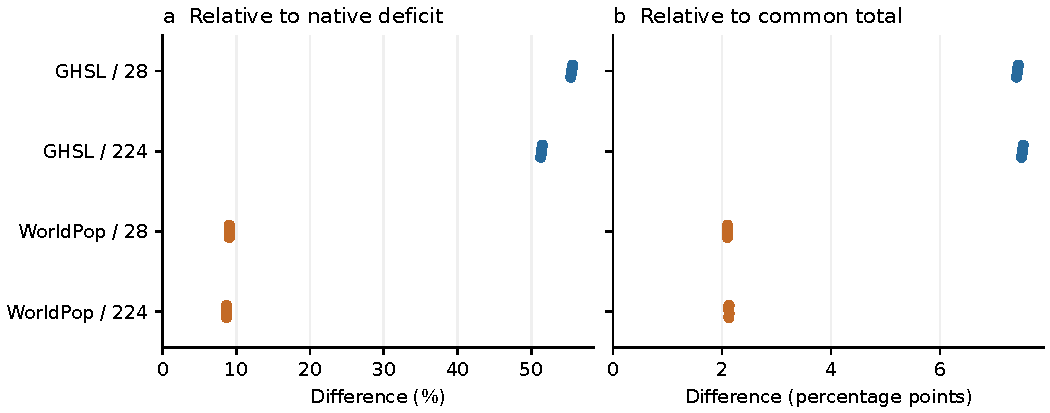
\includegraphics[width=\linewidth]{figures/S5_cross_sensitivity.pdf}
\caption{Crossed aggregation sensitivity. Dots show four grid origins and horizontal lines span them. Left: difference relative to the native-model deficit. Right: the same difference as percentage points of the common population total. Colors identify population model; the 28 and 224 labels identify distinct pair selections.}\label{fig:cross}
\end{figure}

Complete 16-row results, the 25-m comparison, conservation ledger and input SHA-256 values are retained in \path{results/cross_sensitivity/}. The analysis and figure can be regenerated with \path{experiment_cross_sensitivity.py} and \path{make_cross_sensitivity_paper.py}.
